%%%% main.tex — preprint source
\documentclass{article}
\pdfpagewidth=8.5in
\pdfpageheight=11in

\usepackage{ijcai26}

% Use the postscript times font!
\usepackage{times}
\usepackage{soul}
\usepackage{url}
\usepackage[hidelinks]{hyperref}
\usepackage[utf8]{inputenc}
\usepackage[small]{caption}
\usepackage{graphicx}
\usepackage{amsmath}
\usepackage{amsthm}
\usepackage{booktabs}

\urlstyle{same}

\newtheorem{example}{Example}
\newtheorem{theorem}{Theorem}

\pdfinfo{
/TemplateVersion (IJCAI.2026.0)
}

\title{A Probabilistic Decision Framework for CI Failure Diagnosis: Selecting Evidence and Choosing Actions Under Cost Uncertainty}

\author{
    Diwas Pathak
    \affiliations
    Independent Researcher
}

\begin{document}

\maketitle

\begin{abstract}
When a continuous integration (CI) run fails, the true root cause is never directly observable: the agent sees only indirect signals such as which pipeline step failed first, what the fix commit changed, whether a rerun passes, and whether the failure reproduces locally. This paper formulates CI failure diagnosis as sequential decision-making under partial observability. A Bayesian belief over seven hidden root-cause states, with priors counted from 567 real Python CI repair cases, drives an expected-cost comparison over three actions: fix the code, fix the dependency, or escalate to a human. The central question is when the agent should stop gathering evidence and act. Five operating policies are compared on 500 simulated cases. The cost-based value-of-information (VoI) policy is the most accurate (63.0\%) and cheapest (\$35.01 per case): it buys a \$0.07 rerun check only when the answer can change the decision, and never buys a \$33.33 local reproduction whose information never pays for itself. An information-gain heuristic that counts bits but not dollars buys evidence in every case and does not beat belief-only reasoning. Failure analysis shows the remaining errors concentrate where coarse evidence is semantically ambiguous, and three design changes are re-tested, including one negative result.
\end{abstract}

\section{Introduction}

A CI run turns red. Something is broken, but the run itself never states what: a failing test step might be a genuine regression, a flaky test, a dependency that stopped resolving, or a runner with a missing system library. The root cause is a \emph{hidden state} --- one reality, never observed directly --- and the signals a CI system exposes (logs, diffs, reruns) are only indirect evidence about it.

The naive approach is to hand the log to a large language model and ask for the cause. That collapses two decisions that should be separate: what to believe, and what to do. It also ignores two structural facts of the problem. First, evidence is not free. Re-running a pipeline costs compute minutes; asking a developer to reproduce a failure locally costs twenty minutes of expensive human time. An agent that always gathers every piece of evidence wastes money; an agent that never gathers any acts on guesses. Second, errors are asymmetric. A correct automated fix costs a five-minute human spot-check; a wrong one triggers a review--rerun--re-diagnosis chain that costs nine times as much --- and escalating to a human sits between the two. With asymmetric costs, the most \emph{likely} cause is not always the right thing to act on: at 38\% belief that the failure is in code scope, acting is rational; at 37\%, escalating is.

This paper builds and evaluates a small diagnosis agent that reasons the way a careful engineer does: start with a prior belief over root-cause categories, update it with each piece of evidence using Bayes' rule, decide which evidence is worth buying by comparing its cost against the decision value of the information it carries, and act only when acting has the lowest expected cost. The contributions are:

\begin{itemize}
\item a probabilistic model of CI failure diagnosis: seven hidden states with empirical priors from 567 real repair cases, four evidence sources, and a fully assumed-but-labeled cost model;
\item a comparison of five operating policies on 500 reproducible simulated cases, from a majority baseline to a cost-based value-of-information rule;
\item a failure analysis that classifies the most expensive errors, identifies systematic failure modes (coarse evidence that is semantically ambiguous across states), and re-tests three design changes, including one negative result;
\item a generalization analysis that re-derives the decision threshold under catastrophic tails, 10$\times$ evidence prices, and unreliable historical data.
\end{itemize}

Everything is reproducible: the priors and likelihoods come from a public dataset, and every experiment is a standalone script over the same benchmark.

\section{Related Work}

The only academic paper read during this project was Zheng et al.'s empirical study of why GitHub Actions workflows fail \cite{zheng2025gha}. It changed the design in two concrete ways. First, its observation that workflow failures concentrate in specific pipeline stages motivated the first evidence source: the step that fails \emph{first} (install, build, test, lint) is a structural signal about which phase the root cause manifests in, which became E1 in Section~\ref{sec:probabilistic}. Second, its 16-type taxonomy of failure categories was collapsed into the seven hidden states used here, grouped by shared repair action (Appendix~\ref{app:mapping}). One engineering blog post --- Micco's account of how Google detects and mitigates flaky tests \cite{micco2016flaky} --- informed the generalization analysis of Section~\ref{sec:generalization}. Beyond these, the design borrows a structural template --- act / gather information / withhold --- that is standard in clinical decision theory, but no other written source was consulted; the likelihood tables, cost model, and policies were derived from the dataset and from first-principles reasoning about costs, with practitioner input from the discussions in Section~\ref{sec:discussions}.

\section{Probabilistic View of the Agent}
\label{sec:probabilistic}

\subsection{Hidden States and Priors}

The agent models the cause of a failure as one of seven mutually exclusive hidden states, including a residual state for everything the taxonomy does not name. The seven states are a collapse of the 16 failure types in Zheng et al.'s taxonomy of GitHub Actions failures \cite{zheng2025gha}: each state merges the types that share a repair action (unresolved dependencies and dependency conflicts both fix to updated pins, so they form one state; quality-check and vulnerability-scan rejections are both static-tool rejections, so they form another). Appendix~\ref{app:mapping} gives the complete mapping. The states were then populated from the \texttt{error\_type} column of a public dataset of 567 Python CI repair cases collected from real GitHub repositories, with multi-label symptom tags disambiguated to a single primary cause per case --- so the priors below are counted from the Python dataset, not from Zheng et al.'s Java-project frequencies.

The priors are simply the observed frequencies of each state in the dataset --- no smoothing, no external literature (Table~\ref{tab:priors}). The distribution is heavily skewed: static analysis and dependency failures together account for 72.8\% of cases. The prior entropy is
\[
H(S) = -\textstyle\sum_i P(S_i)\log_2 P(S_i) = 2.110 \text{ bits},
\]
so before seeing anything, identifying the cause takes about two yes/no questions' worth of uncertainty.

\begin{table}[t]
\centering
\small
\begin{tabular}{llrr}
\toprule
State & Description & Count & Prior \\
\midrule
S1 & Source code issues & 15 & 0.0265 \\
S2 & Project config issues & 33 & 0.0582 \\
S3 & Dependency failures & 177 & 0.3122 \\
S4 & Static analysis failures & 236 & 0.4162 \\
S5 & Test failures & 66 & 0.1164 \\
S6 & Environment setup issues & 32 & 0.0564 \\
S7 & Other (transient/external) & 8 & 0.0141 \\
\midrule
 & Total & 567 & 1.0000 \\
\bottomrule
\end{tabular}
\caption{Hidden root-cause states and empirical priors, counted from 567 disambiguated CI repair cases.}
\label{tab:priors}
\end{table}

\subsection{Evidence Sources}

The agent can observe four pieces of evidence, two free and two paid:

\begin{itemize}
\item \textbf{E1 --- first failed pipeline step} (free). Which step of the pipeline failed first: install (A), build (B), test (C), static analysis (D), workflow setup (E), or other (F). Extracted from the failed job's step list.
\item \textbf{E2 --- changed files} (free). File categories touched by the change: \texttt{src}, \texttt{test}, \texttt{config}, \texttt{ci}, \texttt{doc}, \texttt{mixed}, or \texttt{none}. In live use this is the diff between the failing commit and the last green commit.
\item \textbf{E3 --- rerun outcome} (\$0.07). Does the identical commit pass if the run is simply retried? Twelve minutes of a hosted runner at \$0.006/min.
\item \textbf{E4 --- local reproducibility} (\$33.33). Does the failure reproduce on a developer's machine? Twenty minutes of developer time at an assumed \$100/hour.
\end{itemize}

The likelihood tables $P(\text{evidence} \mid \text{state})$ for E1 and E2 are empirical cross-tabulations of the 567 cases, with Laplace add-one smoothing so that no observation can zero out a state permanently (full tables in Appendix~\ref{app:likelihoods}). The E3 and E4 tables are \emph{assumed}, not measured: they are reasoned from domain semantics (a syntax error is deterministic and always reproduces locally; a network flake usually clears on rerun and rarely reproduces locally). Table~\ref{tab:e34} shows both; they are labeled as assumptions wherever they are used.

\begin{table}[t]
\centering
\small
\begin{tabular}{lcccc}
\toprule
 & \multicolumn{2}{c}{E3 rerun (assumed)} & \multicolumn{2}{c}{E4 local repro (assumed)} \\
\cmidrule(lr){2-3} \cmidrule(lr){4-5}
State & pass & fail & repro & not \\
\midrule
S1 & 0.05 & 0.95 & 0.92 & 0.08 \\
S2 & 0.05 & 0.95 & 0.80 & 0.20 \\
S3 & 0.15 & 0.85 & 0.45 & 0.55 \\
S4 & 0.03 & 0.97 & 0.90 & 0.10 \\
S5 & 0.35 & 0.65 & 0.40 & 0.60 \\
S6 & 0.50 & 0.50 & 0.25 & 0.75 \\
S7 & 0.75 & 0.25 & 0.15 & 0.85 \\
\bottomrule
\end{tabular}
\caption{Assumed likelihoods for the two paid evidence sources. E3: probability the run passes/fails on rerun. E4: probability the failure does/does not reproduce locally. These are reasoned priors on behaviour, not measured frequencies.}
\label{tab:e34}
\end{table}

\subsection{A Worked Belief Update}

The agent updates beliefs with Bayes' rule after each observation: $P(S_i \mid o) = P(S_i)\,P(o \mid S_i) / P(o)$. A full worked example, by hand:

\paragraph{Step 0.} Beliefs start at the priors of Table~\ref{tab:priors}; entropy 2.110 bits.

\paragraph{Step 1 --- observe E1 = D (the static-analysis step failed first).}
Each state's belief is multiplied by $P(D \mid S_i)$ and renormalised. The normaliser is $Z = 0.3910$. The posterior concentrates on S4:
S4: $0.4162 \times 0.6488 / Z = 0.6907$;
S3: $0.3122 \times 0.3279 / Z = 0.2618$;
all others $\le 0.0124$. Entropy falls from 2.110 to 1.188 bits --- the observation removed 0.922 bits of uncertainty.

\paragraph{Step 2 --- observe E2 = \texttt{src} (only source files changed).}
Multiplying again by $P(\texttt{src} \mid S_i)$ with $Z = 0.4317$: S4 reaches $0.6907 \times 0.5309 / Z = 0.8494$, S3 falls to 0.1220, everything else below 0.01.

\paragraph{Decision.} The action with the lowest expected cost (Section~\ref{sec:policy}) is now \emph{Fix Code}, at an expected cost well below escalation. The agent commits.

\subsection{Where the Threshold Comes From}
\label{sec:threshold}

\paragraph{The same arithmetic in miniature.} An umbrella decides by exactly the equation this section derives, so it is worth doing once on a domestic scale. Say rain tomorrow has probability 0.35. Case A, a normal walk: carrying the umbrella costs 2 units of annoyance, getting wet costs 5. Carrying always costs 2; leaving it costs $0.35 \times 5 = 1.75$ on average --- leave it. The break-even rain chance is $2/(2+5) = 0.40$, and the forecast sits below it. Case B, a wedding in clothes that cannot be replaced: getting wet costs 200, so the break-even is $2/202 \approx 0.01$ and 0.35 is thirty-five times over --- take it. The probability never moved between the cases; the costs decided. The agent's threshold below is this same division with dollar costs.

\paragraph{The agent's cost model} (all values assumed, at an engineer rate of \$100/hour): a \emph{correct} automated fix costs \$8.33 (five-minute human spot-check); a \emph{wrong} automated fix costs \$75.07 (patch review \$25.00 + CI rerun \$0.07 + manual re-diagnosis \$50.00); escalation costs a flat \$50.00 (30 minutes of triage). With $p$ the belief that the failure is a code-scope issue (S1/S2/S4 for \emph{Fix Code}, or S3 for \emph{Fix Dependency}), acting is preferred when
\begin{equation}
p \cdot 8.33 + (1-p) \cdot 75.07 \;<\; 50.00,
\end{equation}
which solves to $p > p^{*} = 25.07 / (25.07 + 41.67) \approx 0.3756$.
The two pieces of the ratio have direct meanings: \$25.07 is how much is wasted by acting when escalation was right, and \$41.67 how much is wasted by escalating when acting was right. The threshold sits at their break-even, not at a round confidence number. It is not knife-edge: perturbing any one cost by $\pm$10\% at a time moves $p^*$ only within $[0.30, 0.45]$. It \emph{is} cost-shaped: if a wrong fix could break production at \$5{,}000 instead of \$75.07, the same algebra gives $p^* = 99.2\%$ --- near-certainty before acting (Section~\ref{sec:generalization} returns to this).

\section{Information-Theoretic View}
\label{sec:info}

This section covers only the information-theoretic concepts the agent actually uses, each with a number from this problem. All logarithms are base 2, so quantities are in bits.

\paragraph{Entropy.} Entropy measures how spread a belief distribution is --- equivalently, the expected number of yes/no questions needed to pin down the truth. The prior over the seven states has $H = 2.110$ bits; after observing E1 = D it drops to 1.188 bits.

\paragraph{Information gain and conditional entropy.} The information gain of an evidence source is the expected drop in entropy from observing it:
$\mathrm{EIG}(E) = H(S) - \sum_o P(o)\, H(S \mid o)$,
where the sum runs over the possible outcomes $o$ and $H(S \mid o)$ is the conditional entropy of the posterior after each outcome. At the prior, EIG(E1) = 0.358 bits and EIG(E2) = 0.173 bits. These are not fixed properties of the sources: evidence gains overlap, and each one shrinks what is left to learn. After E1 = D has already removed 0.922 bits, E2's marginal gain falls to about 0.11 bits --- observing both free sources is expected to remove $0.922 + 0.111 = 1.033$ bits in total from the prior, not 1.033 bits for E2 alone. For free evidence the shrinking marginal does not matter (the price is right either way); for priced evidence it is exactly the point, and Section~\ref{sec:selection} prices it. Information gain is the same quantity as mutual information between the state and the evidence outcome --- how much observing one tells you about the other; unlike correlation, it applies to categorical variables such as these and captures any dependence, not just linear one.

\paragraph{KL divergence.} The Kullback--Leibler divergence $D_{\mathrm{KL}}(P \,\|\, Q) = \sum_x P(x) \log_2 \frac{P(x)}{Q(x)}$ measures how surprised a distribution $P$ will be to see data actually drawn from $Q$. It is not a distance: it is asymmetric and infinite when $Q$ assigns zero probability to something $P$ considers possible. A coin that is always heads, evaluated against a fair coin, gives infinite surprise in one direction and a finite value in the other.

\paragraph{Jensen--Shannon divergence.} Because KL is unbounded and asymmetric, the drift monitor in this project uses the Jensen--Shannon divergence: a symmetrised, smoothed version of KL, bounded in $[0, 1]$ with bits as the base-2 logarithm. It is used to detect distribution shift: comparing the state-prior distribution of the benchmark used for evaluation against a deliberately shifted out-of-distribution benchmark gives $\mathrm{JSD} = 0.2148$, above the 0.05 alert threshold --- a machine-checkable signal that a model calibrated on one population is being applied to another.

\paragraph{Calibration.} A calibrated agent that says ``70\%'' is right about 70\% of the time. Calibration was checked for the best policy by binning its final beliefs per state and comparing mean predicted probability against actual frequency. The agent is well calibrated at the extremes --- in the 80--90\% bin for S4 it predicted 83.9\% and was right 83.2\% of the time (125 cases), and in the dominant 0--10\% bin for S7 it predicted 1.1\% versus 0.8\% actual (492 cases) --- but overconfident in one intermediate band: in the 60--70\% bin for S4 it predicted 63.2\% and was right only 46.7\% of the time (30 cases). Intermediate confidence is exactly where the decision threshold operates, so this miscalibration matters and motivates the uncertainty band in the next section.

\paragraph{Expected cost and value of information.} The expected cost of an action is its average cost if the same decision were repeated many times, weighted by current belief:
$\mathrm{EC}(a) = \sum_s P(s)\, C(a, s)$.
The value of information of a paid evidence source is the expected saving from buying it before acting:
\begin{equation}
\mathrm{VoI}(E) = \min_a \mathrm{EC}(a) \;-\; \Big( c_E + \sum_o P(o) \min_a \mathrm{EC}_o(a) \Big),
\label{eq:voi}
\end{equation}
where $c_E$ is the price of $E$ and the inner term re-optimises the action after each possible outcome $o$. Information has value only if it can change the action, and only if that change saves more than the check costs. In one worked case, the \$0.07 rerun check had $\mathrm{VoI} = +\$3.02$ (bought) while the \$33.33 local reproduction had $\mathrm{VoI} = -\$22.87$ (skipped): the reproduction is more informative in bits, but the belief it would shift is not worth enough dollars to justify its price.

\section{Information Selection}
\label{sec:selection}

The design began with five candidate questions the agent could ask, tabled in the format of expected information value against cost (Table~\ref{tab:candidates}). Four became implemented evidence sources; the fifth --- fingerprinting the actual error line inside the failing log --- is a hypothetical kept from the design table because the failure analysis of Section~\ref{sec:failures} kept pointing at exactly the gap it would fill.

\begin{table*}[t]
\centering
\small
\setlength{\tabcolsep}{5pt}
\begin{tabular}{lllll}
\toprule
Question & Possible answers & Info value & Cost & Would ask? \\
\midrule
Q1 E1 first failed step & install \dots other (A--F) & 0.358 bits (measured) & \$0 & always \\
Q2 E2 changed files & 7 file categories & 0.173 bits (measured) & \$0 & always \\
Q3 E3 rerun outcome & pass / fail & 0.120 bits (assumed) & \$0.07 & only if VoI $>$ 0 \\
Q4 E4 local repro & reproduces / not & 0.210 bits (assumed) & \$33.33 & never at this price \\
Q5 error-line fingerprint (proposed) & exception class/module & unmeasured (hypothetical) & $\approx$\$0 & when S3/S4 tie at a lint step \\
\bottomrule
\end{tabular}
\caption{Five candidate questions from the design stage. Info value is expected information gain at the prior; ``measured'' tables are cross-tabulated from the 567 cases, ``assumed'' tables are reasoned priors (Table~\ref{tab:e34}). Q5 was never implemented --- it needs log text the benchmark does not carry --- so its information value is unmeasured, not zero.}
\label{tab:candidates}
\end{table*}

Table~\ref{tab:evidence} puts the four implemented sources on one scale: how much information each carries at the prior, and what it costs.

\begin{table}[t]
\centering
\small
\begin{tabular}{lrrrl}
\toprule
Evidence & EIG (bits) & Cost & Bits/\$ & Source \\
\midrule
E1 first failed step & 0.358 & \$0 & --- & measured \\
E2 changed files & 0.173 & \$0 & --- & measured \\
E3 rerun & 0.120 & \$0.07 & 1.72 & assumed \\
E4 local repro & 0.210 & \$33.33 & 0.006 & assumed \\
\bottomrule
\end{tabular}
\caption{Evidence comparison at the prior. E1 and E2 are free, so their bits-per-dollar is unbounded; the paid sources are ranked by information per dollar, which inverts their information-only ranking.}
\label{tab:evidence}
\end{table}

The table already exposes the trap this project fell into and then corrected. Ranked by raw information, E4 (0.210 bits) looks better than E3 (0.120 bits). Ranked by information per dollar, they invert completely: E3 delivers 1.72 bits per dollar, E4 delivers 0.006 --- a factor of about 270. A policy that selects evidence by expected information gain (Section~\ref{sec:policy}, P3) buys E4 whenever its marginal bits beat the threshold, and pays \$33.33 for belief movement that rarely changes the action. The correct comparison is not ``how many bits do I get?'' but ``does the expected cost after observing the evidence drop by more than its price?'' --- which is exactly the VoI rule of Equation~\ref{eq:voi}. The free sources are always taken; the paid ones are bought only when their value exceeds their price, and E3's conditional value depends on context: at the prior it removes only 0.120 bits, but after E1 and E2 have already narrowed the field, a pass on rerun is strong evidence for the transient/environment states (S6, S7) and is often exactly the bit that matters.

\section{Decision Policy}
\label{sec:policy}

\paragraph{Action set.} Three actions: \emph{Fix Code} (correct for S1, S2, S4), \emph{Fix Dependency} (correct for S3), and \emph{Escalate} (the only correct response to S5, S6, S7, and the safe default everywhere). Escalation is deliberately modelled as a real action with a real cost, not a failure.

\paragraph{Acting.} Given a posterior, the expected cost of each action is $\mathrm{EC}(a) = \sum_s P(s)\,C(a,s)$ under the cost matrix of Section~\ref{sec:threshold}; the agent picks the argmin. The break-even threshold $p^* = 0.3756$ derived there is the two-action special case of this rule.

\paragraph{Escalation within the band.} Point estimates near the threshold are fragile, so the conservative policy adds an uncertainty band: escalate when the two cheapest actions are within \$5.00 of each other in expected cost, or when no single state reaches 55\% posterior mass. Both numbers were initially guesses; Section~\ref{sec:results} reports a variant that derives them from the cost model instead.

\paragraph{Stop rule.} Free evidence is always observed. For paid evidence, the policies differ:
\begin{itemize}
\item \textbf{P3 (information gain per dollar):} rank pending evidence by $\mathrm{EIG}(E)/c_E$; buy while the score exceeds 0.05 bits/\$, stopping early once the decision leaves the uncertain band. Counts information, never money.
\item \textbf{P4 (value of information):} buy the pending evidence with the highest positive VoI (Equation~\ref{eq:voi}); stop as soon as nothing has positive value. This is the stop rule in its most direct form: act when acting now is cheaper than any evidence-adjusted alternative.
\end{itemize}
If no evidence remains and the posterior still sits in the uncertain band, the agent escalates with a ranked posterior attached to the report --- an agent that must never act silently needs a named safe default, and escalation is this design's.

\section{Experiment}

\paragraph{Setup.} Five policies are evaluated on 500 simulated CI failure cases (seed 42; seeds 7 and 123 used for the robustness check in Section~\ref{sec:results}). Each case is generated by sampling a true hidden state from the empirical priors of Table~\ref{tab:priors}, then sampling each evidence outcome from the likelihood tables conditioned on that state. Every policy runs on the same cases through the same harness, and every case is scored by the same realised cost from the cost matrix.

\paragraph{Policies.}
\textbf{P0} (majority baseline) always outputs the most common action, fit on the evaluation cases themselves --- a slightly optimistic floor.
\textbf{P1} (belief-only) observes the free evidence, picks the most likely state, and takes that state's mapped action; no cost sensitivity, no paid evidence.
\textbf{P2} (expected-cost threshold) minimises expected cost over actions, escalating inside the uncertainty band (\$5.00 gap / 55\% belief); free evidence only.
\textbf{P3} (information gain per dollar) adds evidence buying by the $\mathrm{EIG}/\$$ rule of Section~\ref{sec:policy}.
\textbf{P4} (cost-based VoI) buys paid evidence only when its VoI is positive.

\paragraph{Metrics.} Action accuracy against the ground-truth action implied by the true state; expected cost per case (decision cost + information cost); paid checks per case (questions asked); and escalation rate. Accuracy alone is the wrong metric here --- a policy can be accurate and expensive --- so cost is the primary axis.

\paragraph{Honest circularity note.} The benchmark is sampled from the same likelihood tables the policies reason with. The experiments therefore measure how well each \emph{policy} decides \emph{given} the assumed model; they cannot validate the likelihoods or the cost numbers themselves, which are assumptions, not measurements. Section~\ref{sec:limitations} returns to this.

\section{Results}
\label{sec:results}

\begin{table}[t]
\centering
\small
\setlength{\tabcolsep}{4pt}
\begin{tabular}{lrrrrr}
\toprule
Policy & Acc. & \$/case & Checks & Escal. & E3 bought \\
\midrule
P4 --- cost-based VoI & \textbf{63.0\%} & \textbf{\$35.01} & 0.34 & 17.2\% & 33.8\% \\
P1 --- belief-only & 61.6\% & \$35.57 & 0 & 7.4\% & 0\% \\
P3 --- info-gain/\$ & 60.4\% & \$35.93 & 1.00 & 33.4\% & 100\% \\
P2 --- cost threshold & 51.0\% & \$37.73 & 0 & 44.6\% & 0\% \\
P0 --- majority & 47.8\% & \$43.17 & --- & 0\% & --- \\
\bottomrule
\end{tabular}
\caption{Policy comparison on 500 simulated cases (seed 42). Cost per case includes information cost; ``checks'' is the average number of paid questions asked per case. No policy ever buys E4 at \$33.33 --- its VoI is never positive.}
\label{tab:results}
\end{table}

\begin{figure*}[t]
\centering
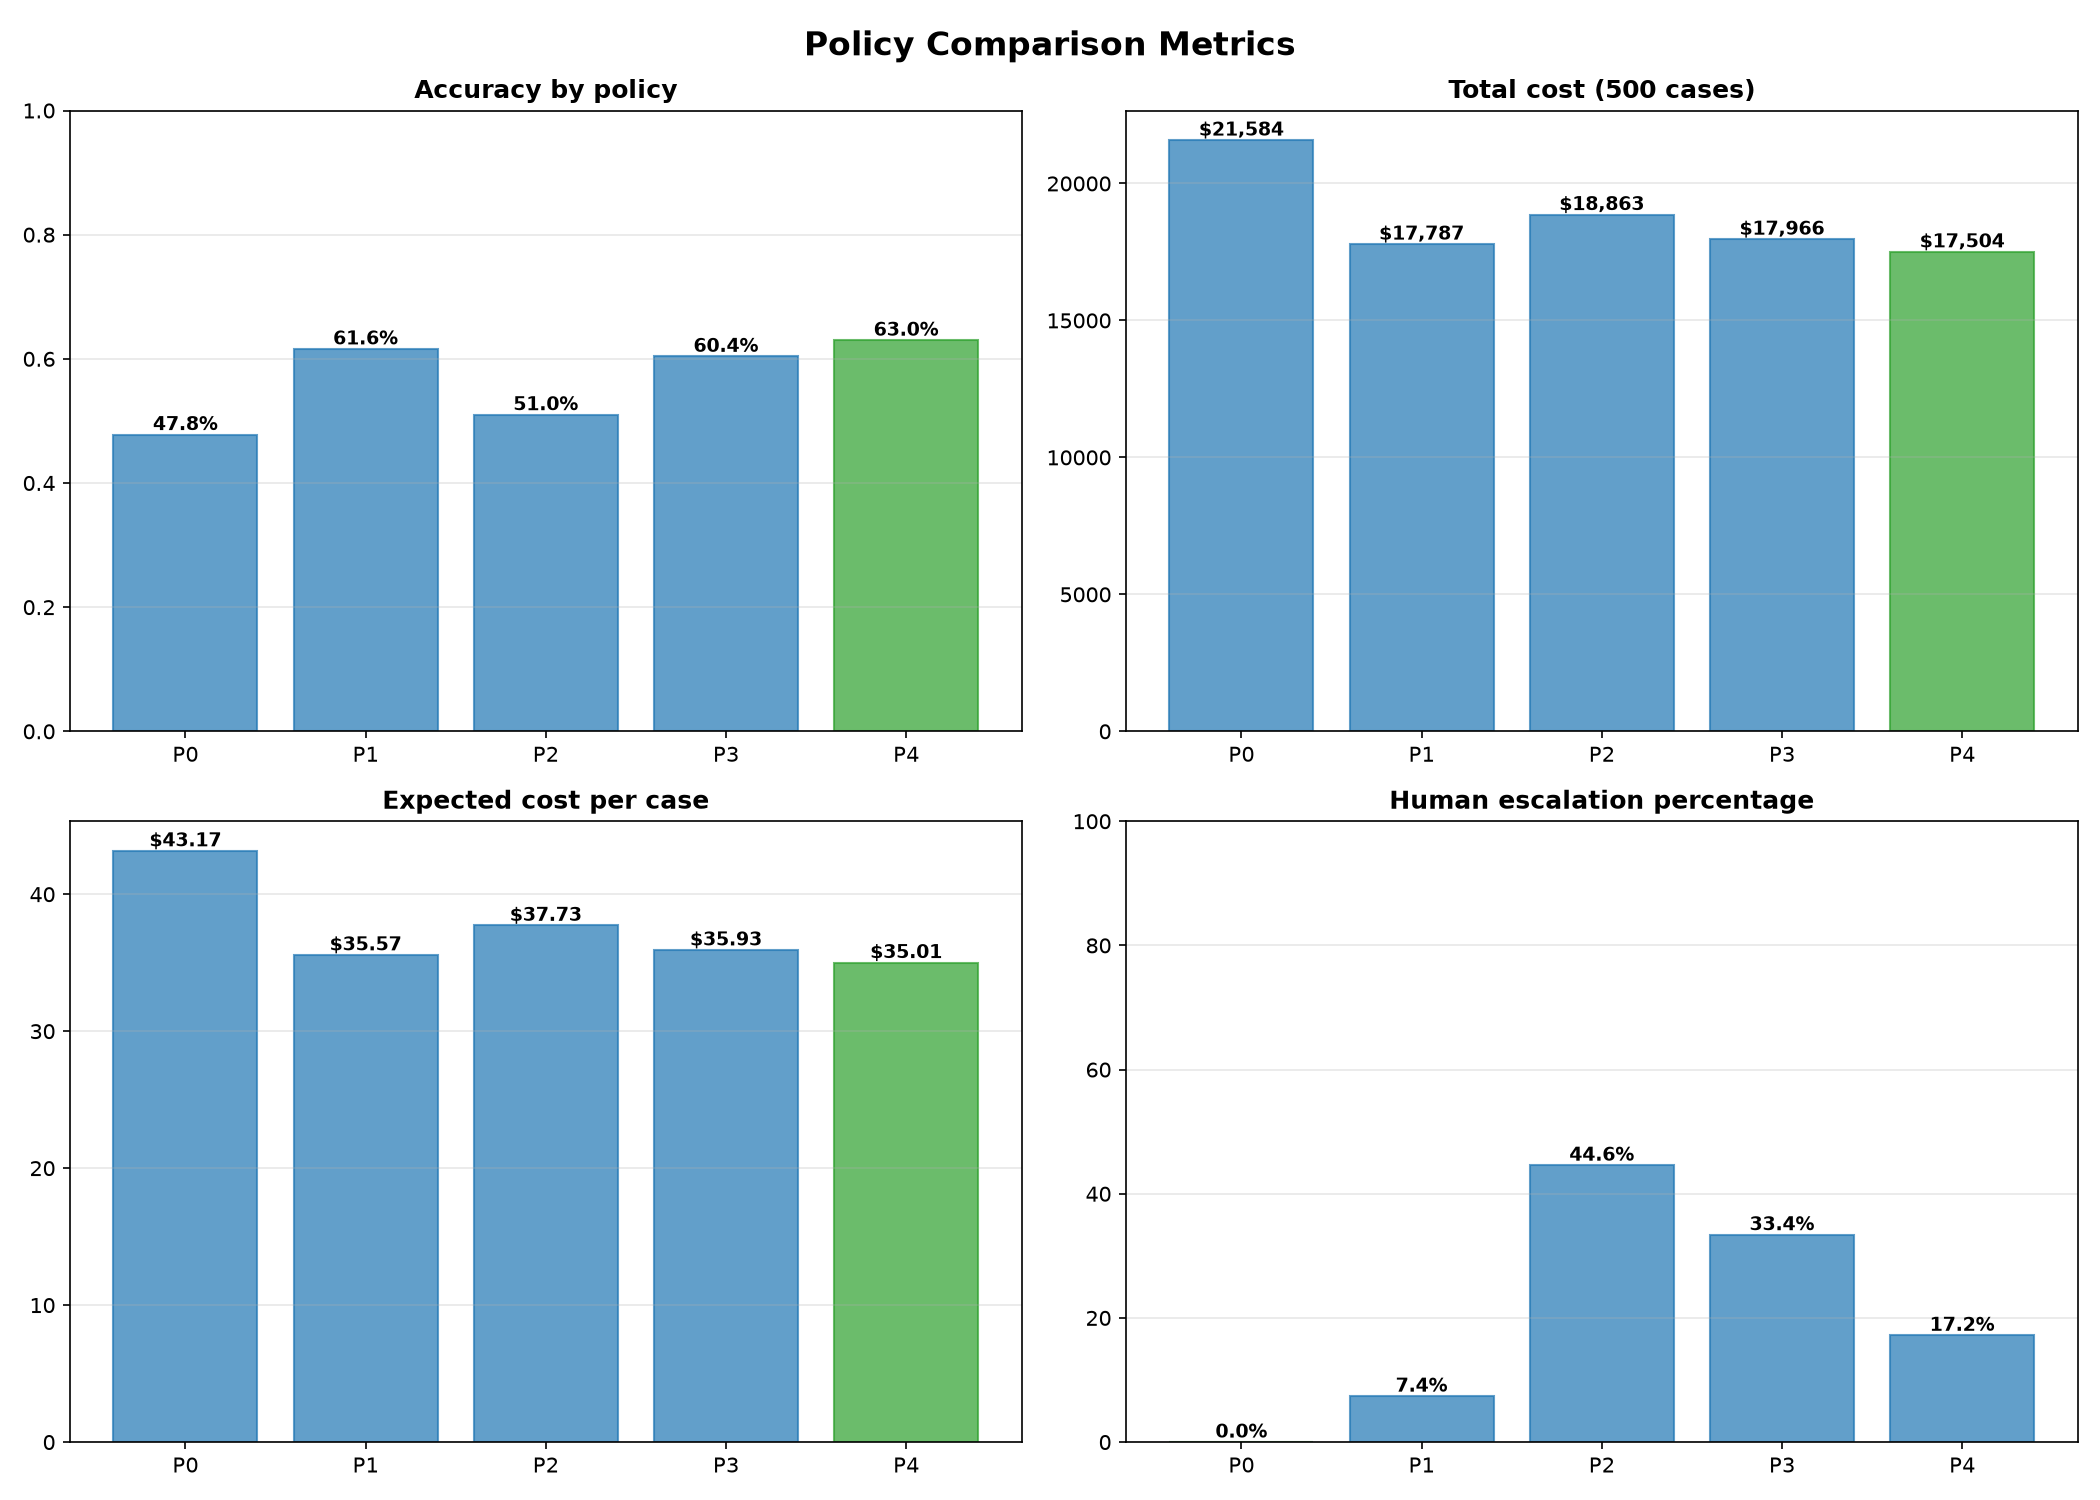
\includegraphics[width=\textwidth]{figures/policy_comparison.png}
\caption{Policy comparison on the seed-42 benchmark: accuracy, total cost over 500 cases, expected cost per case, and escalation rate. The VoI policy (P4, green) dominates on both accuracy and cost.}
\label{fig:comparison}
\end{figure*}

Table~\ref{tab:results} and Figure~\ref{fig:comparison} show the headline comparison. Three findings:

\textbf{The VoI rule wins on both axes.} P4 is simultaneously the most accurate (63.0\%) and the cheapest (\$35.01 per case). Its advantage over belief-only P1 is exactly the paid-evidence decision: it buys the cheap rerun check in the 33.8\% of cases where the rerun answer could change the action, and skips it otherwise. Its information spend is \$0.02 per case against P3's \$0.07 --- for a better result.

\textbf{Information gain per dollar is not value.} P3 buys E3 in 100\% of cases, including the two-thirds where the extra bit cannot flip the decision. The result is worse accuracy than P1 (60.4\% vs 61.6\%) \emph{and} higher cost: buying information that cannot change the action is pure waste, and the extra evidence can even reinforce a wrong belief (Section~\ref{sec:failures}).

\textbf{Conservatism is expensive too.} P2's guessed uncertainty band escalates 44.6\% of cases --- two and a half times as often as P4, and six times as often as the derived-threshold policy of Table~\ref{tab:whatif} --- and lands at 51.0\% accuracy. Escalation is safe, but as a blanket policy it costs more than the wrong actions it avoids.

\subsection{Robustness Across Benchmark Draws}

\begin{table}[t]
\centering
\small
\begin{tabular}{lrr}
\toprule
Policy & Accuracy & \$/case \\
\midrule
P4 --- cost-based VoI & \textbf{63.8\%} $\pm$ \textbf{0.7\%} & \textbf{\$34.21} $\pm$ \textbf{0.57} \\
Fix3 --- derived threshold & 63.3\% $\pm$ 0.4\% & \$39.03 $\pm$ 0.78 \\
P1 --- belief-only & 60.3\% $\pm$ 0.9\% & \$35.96 $\pm$ 0.30 \\
P3 --- info-gain/\$ & 60.0\% $\pm$ 0.7\% & \$35.64 $\pm$ 0.21 \\
P2 --- cost threshold & 50.9\% $\pm$ 0.4\% & \$37.53 $\pm$ 0.25 \\
P0 --- majority & 49.5\% $\pm$ 1.2\% & \$42.01 $\pm$ 0.83 \\
\bottomrule
\end{tabular}
\caption{Mean $\pm$ population standard deviation across three independently sampled 500-case benchmarks (seeds 42, 7, 123); the spread reflects sampling noise between draws, not a confidence interval. The ranking is stable; P4 is the most accurate policy on every seed.}
\label{tab:seeds}
\end{table}

Re-running on two fresh 500-case draws (Table~\ref{tab:seeds}) keeps the ranking intact, so the headline result is not a single-draw artefact.

\subsection{Three Design Changes, Re-tested}

The failure analysis of Section~\ref{sec:failures} motivated three design changes, each re-tested under the identical harness (Table~\ref{tab:whatif}).

\begin{table}[t]
\centering
\small
\begin{tabular}{lrrr}
\toprule
Variant & Acc. & \$/case & Escal. \\
\midrule
P4 baseline & 63.0\% & \$35.01 & 17.2\% \\
Fix 1: E4 priced at \$0.10 & \textbf{68.4\%} & \textbf{\$32.10} & 11.4\% \\
Fix 2: optimistic E3 likelihood & 61.6\% & \$35.46 & 8.6\% \\
Fix 3: derived threshold $p^*$ & 63.8\% & \$39.55 & 7.0\% \\
\bottomrule
\end{tabular}
\caption{Re-tests of the three design changes on the same 500 cases. Fix 2 is a negative result: more trusting rerun beliefs made the policy worse.}
\label{tab:whatif}
\end{table}

\textbf{Fix 1 --- what if local reproduction got cheap?} E4's \$33.33 price is developer time; automating it (e.g., a hosted repro environment) could cut the price to \$0.10. The what-if injects the new price into the VoI rule without touching shared constants. The policy's behaviour inverts completely: it buys E4 in 191 of 500 cases, gaining 5.4 points of accuracy \emph{and} \$2.91 per case. The evidence was never useless --- it was mispriced. This is the clearest single insight of the project: whether information is worth buying is a statement about a price, not about the information.

\textbf{Fix 2 --- what if reruns clear dependency failures? (negative result)} A what-if on beliefs rather than prices: if $P(\text{pass on rerun} \mid S3)$ were 0.40 instead of the assumed 0.15 (flaky mirrors, restored caches), the policy buys E3 twice as often (70.8\%) and escalates less than half as often (8.6\%) --- and accuracy \emph{drops} 1.4 points while cost \emph{rises} to \$35.46 per case. Believing the world is friendlier than the model says produces over-confident acting. Mis-specified beliefs cost more than the extra evidence they justify. This experiment also surfaced a real data bug: the benchmark stored the rerun outcome under a column the original notebook never read, so E3 was silently updating nothing until the mapping was fixed.

\textbf{Fix 3 --- thresholds derived, not guessed.} P2's \$5.00 gap and 55\% confidence were guesses; the break-even $p^* = 0.3756$ of Section~\ref{sec:threshold} is derived from the same costs. A policy that gathers evidence one piece at a time until a fix action's correct-belief mass clears $p^*$ reaches 63.8\% accuracy --- the best of all variants --- with the lowest escalation rate (7.0\%). But it costs \$39.55 per case, because its evidence-buying rule (like P3's) still buys the \$33.33 local repro in 74 cases where the belief gain never pays for itself. The threshold layer is an improvement; the evidence-buying layer still needs VoI. Combining Fix 3's acting rule with P4's buying rule is the obvious next design, left open in Section~\ref{sec:newquestions}.

\section{Failure Analysis}
\label{sec:failures}

P4 misclassifies 185 of 500 cases (63.0\% accuracy). The five most expensive failures all cost \$75.07 --- the wrong-action penalty --- and four of the five share one mechanism. Each was traced belief-by-belief with a dry-run of the update chain, answered with a ten-question diagnostic (what did the agent believe; what was true; which evidence was used, ignored, or unaffordable; was the probability, the state list, the threshold, or the cost model at fault; should a human have been involved), and classified.

\textbf{Failures 1, 3, 4 (cases 0, 17, 18) --- a dependency failure crashing the lint step. \emph{Classification: misleading evidence + systematic bias.}} The true state is S3 (dependency failure), but the first failed step is the static-analysis step (E1 = D), because a missing dependency makes lint tools crash on import. The belief trace is identical in all three: priors $\to$ E1 = D pushes S4 to 0.691 $\to$ E2 = \texttt{mixed} lands at S4 0.533 / S3 0.422 $\to$ the rerun check is bought (its VoI is positive) but \emph{fail on rerun} is consistent with both S3 and S4, so it \emph{reinforces the wrong belief} (S4 rises to 0.569) $\to$ E4 would disambiguate but its VoI is $-\$22.87$ $\to$ \emph{Fix Code}, wrong. Three independent failures with the same trace make this a systematic blind spot of coarse evidence, not bad luck: whenever a dependency failure manifests at a lint step, the model prefers the wrong explanation.

\textbf{Failure 2 (case 10) --- an environment failure crashing the test step. \emph{Classification: misleading evidence.}} The true state is S6 (missing system library), but the pytest step fails first (E1 = C), which reads as a dependency or test failure. Posterior: S3 0.553, S6 only 0.099. Both paid checks are skipped (negative VoI), and the agent takes \emph{Fix Dependency}. Escalation, the only correct action for S6, would have saved \$25.07.

\textbf{Failure 5 (case 23) --- a test failure behind a workflow-step error and a \texttt{src} diff. \emph{Classification: misleading evidence + insufficient information.}} E1 = E (workflow) with E2 = \texttt{src} points at static analysis (S4 reaches 0.579 after the rerun check); the true state is S5 (test failure), for which escalation was required. The local repro --- the one check that separates these states --- was again unaffordable at \$33.33.

\paragraph{What changed.} The analysis exposed three weaknesses and each produced a re-tested change: (1) E4 is the designated disambiguator for exactly these failure pairs, but priced out of every case --- hence Fix 1, which showed that at \$0.10 the same policy buys it and recovers most of these errors (68.4\% accuracy); (2) no single cheap evidence separates S3 from S4 when the failure surfaces at a lint step, motivating finer-grained evidence (candidate Q5, the error-line fingerprint of Table~\ref{tab:candidates}) rather than more thresholds; (3) the benchmark bug where E3's outcome column was never read was found by noticing that rerun evidence never changed any belief. The residual failure mode that no current change fixes: coarse categorical evidence cannot distinguish states that manifest identically at pipeline granularity.

\section{Human Discussions}
\label{sec:discussions}

Practitioner discussions (recorded across several Reddit communities) shaped two concrete parts of the design; only changes that were actually implemented are reported here.

\textbf{Evidence sources taken from practitioners' triage habits.} Describing their own triage in r/devops, engineers said the first split is ``did it die in my tests or in the plumbing before them,'' that they read the \emph{first} error in the log rather than the last (CI logs cascade), that they weight the diff before anything else, and that the stopping condition is blunt: ``I only call it sure once I can reproduce the failure locally on demand.'' Another respondent's definition of flaky --- ``it works after just running it again'' --- made the rerun a checkable signal. This thread directly produced three of the four evidence sources in this paper: E2 (changed files), E3 (rerun outcome), and E4 (local reproducibility), with E4's role as the pre-commit disambiguator coming from the ``reproduce locally = sure'' heuristic.

\textbf{Removing a hidden state that could not be actionable.} When an earlier version of the state list was posted for review, respondents flagged the \emph{shared-root-cause} hypothesis (``multiple failures, one cause'') as a relationship between failures rather than a standalone cause an agent can act on --- deducing it never changes what you do next. The state list was redesigned accordingly into the seven mutually exclusive states of Table~\ref{tab:priors} (with a residual state), and co-occurrence between causes was dropped from the model rather than represented.

Other suggestions from the same discussions --- a dedicated human-error check, per-hypothesis evidence checklists, and state-dependent escalation costs --- were recorded in the discussion log but not implemented in this system.

\section{Generalization Challenge}
\label{sec:generalization}

The brief decision-theoretic question is: what happens if the world changes? Three stress tests, plus an environment change.

\paragraph{One variable at a time.}
\emph{(1) The cost of a wrong fix becomes catastrophic.} If a wrong patch can break production at \$5{,}000 instead of \$75.07, the break-even of Section~\ref{sec:threshold} moves from $p^* = 0.376$ to $p^* = 0.992$: the agent must be virtually certain before acting, and beyond some stakes escalation should be a structural override (``always a human when state S3 could touch production'') rather than an expected-cost outcome. The action set survives; the autonomy does not.
\emph{(2) Evidence becomes 10$\times$ more expensive.} Re-running P4 with every evidence price multiplied by ten leaves its behaviour \emph{unchanged}: it still buys E3 in exactly the same 33.8\% of cases, with identical accuracy --- only \$0.21 per case more expensive. The buy/no-buy boundary is price-robust because VoI gaps are large: a check worth \$3.02 of expected saving at \$0.07 is still worth buying at \$0.70. The only price that ever mattered in this cost structure is E4's, which is three orders of magnitude above its value (Fix 1).
\emph{(3) Historical data becomes unreliable.} The priors were learned from data; if the world drifts, they are silently wrong. The JSD monitor of Section~\ref{sec:info} is the detector --- the shifted benchmark is flagged at $\mathrm{JSD} = 0.2148$ against the 0.05 threshold --- and the safe behaviour while a drift is unresolved is to fall back on free evidence and escalate more, never to keep acting on stale beliefs. Wiring the monitor into the policy loop (rather than reporting it alongside) is left open in Section~\ref{sec:newquestions}.

\paragraph{Change the environment.} Moving this design from open-source Python CI to a large enterprise breaks assumptions faster than it changes parameters. Priors shift (config and environment issues rise; flakiness grows with suite size --- at Google, roughly one in seven tests exhibits some flakiness \cite{micco2016flaky}, so S7's mass grows). E4 largely disappears: local reproduction of a multi-service stack is often impossible, which removes the designated disambiguator precisely where failure states interleave more. At least one hidden state is missing (compliance or security-policy rejections), and the flat \$50 escalation understates multi-team triage. The threshold itself is the most portable part --- the break-even equation transfers with new costs --- while the state list and the evidence menu are the parts that would need redesign.

\section{Limitations}
\label{sec:limitations}

\paragraph{The evaluation is circular by construction.} Cases are sampled from the same priors and likelihoods the policies use, so the experiments compare decision rules \emph{given} the assumed model. They cannot validate the likelihood tables or the cost numbers against real failures. A deliberate next step is mis-specifying the simulator relative to the agent's model to measure robustness, rather than assuming both match.

\paragraph{Two of four likelihood tables are assumptions.} E1 and E2 are measured from 567 real cases; E3 and E4 are reasoned from domain semantics, not measured. The Fix 2 experiment shows exactly how sensitive the policy is to getting one such number wrong.

\paragraph{All costs are assumed.} The \$100/hour rate, \$75.07 wrong-fix chain, flat \$50.00 escalation, and 20-minute local repro are a coherent first model, not measurements. The flat wrong-fix cost in particular hides fat tails: some wrong patches break other pipelines and cost far more than \$75.07 --- Section~\ref{sec:generalization} quantifies what those tails do to the threshold.

\paragraph{The state list is both too coarse and too rigid.} Coarse evidence cannot separate states that manifest identically (S3 vs.\ S4 at a lint step --- the dominant failure mode in Section~\ref{sec:failures}). And mutual exclusivity is a modelling convenience: real CI failures stack (a dependency break plus a flaky test), and the posterior then concentrates on a single wrong cause with high confidence. S1 and S7 likelihoods are smoothing-dominated (15 and 8 rows) and should be treated as placeholders.

\paragraph{Transfer and deployment.} Priors come from open-source Python CI and will not transfer directly to enterprise codebases (Section~\ref{sec:generalization}). Conditional independence of E1 and E2 given the state is assumed but violated in reality, likely making posteriors overconfident. Nothing here has been deployed: the 17.2\% escalation rate and the mandatory human verification of every automated patch are the standing human oversight, and both would need live measurement before any autonomous use.

\section{New Questions}
\label{sec:newquestions}

The results raised questions the project cannot yet answer.

\begin{enumerate}
\item How should an agent behave when the true failure is a \emph{combination} of states its mutually exclusive list cannot express, given that the failure analysis shows the posterior then concentrates confidently on one wrong cause?
\item Does a more granular hidden-state list, by itself, ensure that the root cause of a complex CI run can be caught? The failure analysis suggests not: the dominant errors came not from missing states but from coarse evidence unable to separate states already in the list (Section~\ref{sec:failures}), which suggests evidence granularity matters at least as much as state granularity.
\item What is the right policy response once the JSD monitor fires? The drift alarm detects that the world moved (Section~\ref{sec:generalization}), but the agent has no measured rule for how much to widen its uncertainty band --- or how quickly to re-estimate priors --- while the alarm is active.
\end{enumerate}

\section*{AI-Use Statement}

I used AI to find technical terms for the CI-diagnosis agent, recommend me relevant communities to discuss, to explain KL divergence and Jensen--Shannon divergence in simple language, and to debug the simulation code. I wrote the hidden-state model, the likelihood tables --- with the help of the dataset for the two empirical evidences (E1, E2) and as assumed values for E3 and E4 --- and the cost assumptions myself. I ran the simulation with a coding agent and I verified the results; the results in Table~\ref{tab:results} are from 500 simulated cases. I verified the entropy and KL calculations for all states in Section~\ref{sec:info} before trusting the code. The abstract was drafted with AI assistance and rewritten by me.

\bibliographystyle{named}
\bibliography{references}

\appendix

\section{Core Concepts in Plain Words}
\label{app:concepts}

\begin{enumerate}
\item \textbf{What is a hidden state, and what are yours?} The one real cause behind an observation, which is never seen directly --- only evidence about it is. Mine are the seven root-cause categories of Table~\ref{tab:priors}: source code, project config, dependency, static analysis, test, environment, and a residual ``other''.
\item \textbf{Why is directly predicting an answer sometimes insufficient?} A one-shot prediction throws away how sure the agent is and what different mistakes cost. With belief over states, the agent can update as evidence arrives and can choose to gather more or escalate instead of committing.
\item \textbf{What is a belief distribution, and why must it sum to one?} A belief distribution spreads confidence across the possible causes. It must sum to one because the state list claims to cover every possibility --- if it summed to less, some reality would be missing from the model, which is why a residual state exists.
\item \textbf{What is the difference between prior and posterior?} The prior is confidence before evidence (here: how often each cause appears in 567 real cases); the posterior is the updated confidence after evidence, prior times likelihood renormalised.
\item \textbf{What is likelihood, and how does it differ from probability?} A likelihood $P(\text{evidence} \mid \text{state})$ answers ``if the cause were S4, how often would the lint step fail first?'' --- a property of the evidence channel. The posterior $P(\text{state} \mid \text{evidence})$ answers the diagnostic question. Bayes' rule converts the first into the second.
\item \textbf{What does it mean for an agent to be uncertain?} Its belief is not concentrated: after free evidence, no single state holds enough mass to act on, and no cheap evidence can concentrate it further.
\item \textbf{What is entropy, and why does it represent uncertainty?} The expected surprise of an outcome under the belief distribution --- equivalently, the average number of yes/no questions needed to resolve the truth. My prior has 2.110 bits; after E1 = D, 1.188.
\item \textbf{What is a bit, in plain words?} The unit of entropy: one bit is the uncertainty of a fair coin flip, resolved by one yes/no question. 2.110 bits means about two such questions' worth of unresolved uncertainty.
\item \textbf{What is information gain, and how does it relate to entropy?} The expected drop in entropy from observing a source: EIG = $H$ before minus expected $H$ after. E1 gives 0.358 bits at the prior.
\item \textbf{What is conditional entropy?} The entropy of the belief distribution \emph{after} a specific observation, averaged over observations weighted by their probability --- the $H(S \mid o)$ term inside the EIG sum.
\item \textbf{What is mutual information, and how does it differ from correlation?} The same quantity as information gain: how much observing one variable reduces uncertainty about the other. Unlike correlation it works on categorical variables (my states and outcomes are all categorical) and captures non-linear dependence.
\item \textbf{What is KL divergence, and why is it not a distance?} How surprised distribution $P$ will be sampling data that actually follows $Q$; zero when they match. Not a distance because it is asymmetric --- $D_{\mathrm{KL}}(P\|Q) \neq D_{\mathrm{KL}}(Q\|P)$ --- and unbounded.
\item \textbf{Why is KL divergence asymmetric? Give a small example.} A coin that always lands heads, judged against a fair coin: small finite surprise. Reverse the roles: a fair coin judged against the always-heads coin is \emph{infinitely} surprised the moment tails appears. The two directions measure different mistakes.
\item \textbf{What is Jensen--Shannon divergence, and why was it introduced?} A symmetrised, bounded version of KL (in $[0,1]$ with base-2 logs), introduced because KL's asymmetry and infinity make it awkward as a similarity score. I use it for drift detection: 0.2148 between my benchmark's state distribution and a shifted one, past the 0.05 alert.
\item \textbf{What is calibration, and why does it matter for an agent?} Whether ``70\%'' events actually happen about 70\% of the time. My agent is well calibrated at the extremes (83.9\% predicted vs 83.2\% actual in one high bin) but overconfident mid-range (63.2\% vs 46.7\%) --- and the mid-range is where the acting threshold lives.
\item \textbf{What is expected cost, and how did you derive your threshold from it?} The belief-weighted average cost of taking an action repeatedly. I derived the threshold by equating the expected cost of acting, $p \cdot 8.33 + (1-p) \cdot 75.07$, with the \$50.00 escalation cost, giving the break-even $p^{*} \approx 0.3756$.
\item \textbf{What is value of information? When is more information not worth it?} The expected saving from buying evidence before acting: current best expected cost minus (price + expected best cost after observing it). Not worth it when its price exceeds that saving --- my \$33.33 local repro has negative VoI in every one of the 500 cases at that price.
\item \textbf{Can a question be highly informative and still useless? Give your own example.} Yes: E4 is the most informative paid source in bits (0.210) and useless at \$33.33, because the belief it moves is not worth the price --- 0.006 bits per dollar. Its information only becomes valuable when the price drops (Fix 1).
\item \textbf{What is distribution shift, and how would your agent detect it?} The world's distributions drifting away from the ones the model was built on. I detect it by computing the Jensen--Shannon divergence between the state/evidence distributions of incoming cases and the reference distributions, alerting past a threshold.
\item \textbf{When should your agent stop searching and act? State the rule.} Free evidence is always taken. For paid evidence: buy only while the highest VoI is positive; act when acting now is cheaper than the best evidence-adjusted alternative --- and escalate instead of acting whenever the posterior sits in the uncertainty band.
\end{enumerate}

\section{Empirical Likelihood Tables}
\label{app:likelihoods}

Tables~\ref{tab:e1} and~\ref{tab:e2} give the empirical likelihoods $P(\text{evidence} \mid \text{state})$ for the two free evidence sources: cross-tabulations of the 567 disambiguated cases with Laplace add-one smoothing and row renormalisation.

\begin{table}[h]
\centering
\small
\setlength{\tabcolsep}{4pt}
\begin{tabular}{lcccccc}
\toprule
State & A & B & C & D & E & F \\
\midrule
S1 & 0.048 & 0.095 & 0.476 & 0.143 & 0.095 & 0.143 \\
S2 & 0.231 & 0.026 & 0.436 & 0.077 & 0.077 & 0.154 \\
S3 & 0.169 & 0.016 & 0.443 & 0.328 & 0.016 & 0.027 \\
S4 & 0.025 & 0.008 & 0.079 & \textbf{0.649} & 0.025 & 0.215 \\
S5 & 0.042 & 0.042 & \textbf{0.653} & 0.042 & 0.056 & 0.167 \\
S6 & 0.053 & 0.053 & \textbf{0.684} & 0.079 & 0.053 & 0.079 \\
S7 & 0.143 & 0.071 & \textbf{0.571} & 0.071 & 0.071 & 0.071 \\
\bottomrule
\end{tabular}
\caption{E1 --- first failed pipeline step. Outcomes: A install, B build, C test, D static analysis, E workflow/env, F other. The dominant entry per row is bold; C is dominant for five of seven states, which makes it a weak discriminator.}
\label{tab:e1}
\end{table}

\begin{table}[h]
\centering
\small
\setlength{\tabcolsep}{3.5pt}
\begin{tabular}{lccccccc}
\toprule
State & src & test & cfg & ci & doc & mixed & none \\
\midrule
S1 & \textbf{0.409} & 0.182 & 0.046 & 0.046 & 0.046 & 0.227 & 0.046 \\
S2 & 0.125 & 0.100 & 0.075 & 0.025 & 0.025 & \textbf{0.600} & 0.050 \\
S3 & 0.201 & 0.027 & 0.027 & 0.011 & 0.005 & \textbf{0.723} & 0.005 \\
S4 & \textbf{0.531} & 0.095 & 0.012 & 0.004 & 0.008 & 0.346 & 0.004 \\
S5 & 0.219 & \textbf{0.315} & 0.014 & 0.014 & 0.014 & 0.411 & 0.014 \\
S6 & \textbf{0.359} & 0.077 & 0.026 & 0.026 & 0.026 & 0.462 & 0.026 \\
S7 & 0.067 & \textbf{0.400} & 0.067 & 0.067 & 0.067 & 0.267 & 0.067 \\
\bottomrule
\end{tabular}
\caption{E2 --- changed files in the fix commit. The \texttt{mixed} outcome dominates for S2 and S3 (dependency fixes typically touch a lockfile and source files at once), which limits E2's power for exactly the states that most often co-occur with S4.}
\label{tab:e2}
\end{table}

\section{State List Provenance: Mapping from Zheng et al.'s Taxonomy}
\label{app:mapping}

Zheng et al. \cite{zheng2025gha} manually analyse 375 failed GitHub Actions runs from 260 open-source Java projects and classify them into 16 failure types (P1--P8 project-related, W1--W8 workflow-related). The seven hidden states of this paper are a collapse of those 16 types, grouped by shared repair action. Table~\ref{tab:mapping} gives the complete mapping with the paper's own counts.

\begin{table}[h]
\centering
\small
\setlength{\tabcolsep}{4pt}
\begin{tabular}{llrl}
\toprule
Type & Failure & Count & State \\
\midrule
P1 & source code defects & 54 & S1 \\
P2 & project configuration & 19 & S2 \\
P3 & unresolved dependencies & 33 & S3 \\
P4 & dependency conflicts & 45 & S3 \\
P5 & quality-check failures & 26 & S4 \\
P6 & vulnerability findings & 15 & S4 \\
P7 & performance degradation & 3 & S7 \\
P8 & test failures & 120 & S5 \\
W1 & runner resource limits & 2 & S7 \\
W2 & workflow config errors & 21 & S7 \\
W3 & network issues & 10 & S7 \\
W4 & environment setup failures & 13 & S6 \\
W5 & permission issues & 2 & S7 \\
W6 & unresolvable actions & 3 & S7 \\
W7 & API rate limits & 3 & S7 \\
W8 & version-control issues & 6 & S7 \\
\bottomrule
\end{tabular}
\caption{Mapping from the 16 failure types of Zheng et al.\ (their Figures 3--4; counts are their manually analysed Java-project failures, totalling 375) to this paper's hidden states. States merge types that share a repair action: S3~$=$~P3$+$P4 (both fixed by updating pins or regenerating lockfiles), S4~$=$~P5$+$P6 (both are static-tool rejections fixed in code), and S7 is the residual for causes with no shared automated fix. An earlier 8-state variant kept W2 as its own state; it contained zero cases in the Python dataset (every configuration error there was project-level, not workflow-YAML authoring) and was folded into S7. The priors of Table~\ref{tab:priors} are counted from the 567-case Python dataset after its error-type tags are mapped through the same state list --- not from these Java frequencies, which differ substantially (e.g., test failures are 32\% in Java but 11.6\% here).}
\label{tab:mapping}
\end{table}

\end{document}
